\documentclass[a4paper, 12pt]{article}

\usepackage{graphicx}
\usepackage{subfigure}
\usepackage{hyperref}
\usepackage{xepersian}
\settextfont{XB Niloofar}

\begin{document}

\title{نوروز در حرکت؛\\ تحلیل تردد جاده‌ای و گردشگری در ایران}
\author{گروه کفش مردانهٔ ورزشی}
\date{اسفند ۱۴۰۳}
\maketitle

\section{مقدمه}
نوروز به عنوان یکی از مهم‌ترین رویدادهای فرهنگی ایران، هر ساله باعث افزایش قابل‌توجه تردد جاده‌ای می‌شود. این پدیده نه تنها بر سیستم حمل‌ونقل تأثیرگذار است، بلکه چالش‌ها و فرصت‌هایی در حوزه‌هایی مانند گردشگری، مدیریت ترافیک و برنامه‌ریزی زیرساختی ایجاد می‌کند. تحلیل داده‌های تردد در این بازه، اطلاعات ارزشمندی برای بهبود مدیریت ترافیک، شناسایی مقاصد گردشگری پرطرفدار و توسعه زیرساخت‌ها در اختیار نهادهای دولتی و سرمایه‌گذاران خصوصی قرار می‌دهد.

\section{اهداف پژوهش}
این پروژه به دنبال پاسخ به سوالات زیر است:
\begin{enumerate}
    \item الگوی تردد در بازه نوروز چگونه است؟
        \begin{itemize}
            \item پیک سفرهای نوروزی در چه روزهایی اتفاق می‌افتد؟
            \item کدام مناطق کشور بیشترین حجم تردد را دارند؟
        \end{itemize}
    \item مقاصد گردشگری پرطرفدار کدامند؟
        \begin{itemize}
            \item کدام شهرها بیشترین گردشگر را جذب می‌کنند؟
            \item کدام شهرها بیشترین تعداد گردشگر را به سایر مناطق می‌فرستند؟
        \end{itemize}
    \item چه عواملی در جذب گردشگر تأثیرگذارتر هستند؟
\end{enumerate}

\section{داده‌های مورد استفاده}
برای این پژوهش از منابع داده‌ای مختلفی استفاده خواهیم کرد:
\begin{itemize}
    \item \textbf{داده‌های تردد شمارها:} عمدتاً داده‌های روزانه مورد بررسی قرار می‌گیرند، اما در برخی موارد ممکن است از داده‌های ساعتی نیز برای تعیین نقش شهرها به عنوان مقصد یا گذرگاه استفاده شود. متغیرهای مورد نیاز شامل تعداد وسایل نقلیه کلاس ۱، تعداد کل، تعداد برآورد شده و سرعت متوسط هستند. محدوده جغرافیایی در ابتدا کل کشور را دربرمی‌گیرد و سپس بر اساس نتایج اولیه محدود خواهد شد.
    \item \textbf{وضعیت جاده‌ها:} داده‌های مربوط به وضعیت جاده‌ها از وبسایت سازمان راهداری\footnote{\url{https://rmto.ir/fa/}} به دست خواهند آمد.
    \item \textbf{داده‌های آب‌وهوا:} اطلاعات مربوط به شرایط جوی از طریق وبسایت \lr{Meteostat}\footnote{\url{https://meteostat.net/en/}} به دست خواهد آمد، زیرا دریافت داده از سازمان هواشناسی نیازمند مجوزهای خاص است.
    \item \textbf{اطلاعات اقامتگاه‌ها و هتل‌ها:} این داده‌ها نیز به علت عدم وجود در منابع رسمی، از طریق وبسایت‌های اقامت۲۴\footnote{\url{https://www.eghamat24.com}} و جاباما\footnote{\url{https://www.jabama.com/}} استخراج خواهند شد.
\end{itemize}

در صورت نیاز به داده‌های تکمیلی، از منابع دیگر نیز استفاده خواهد شد.

\begin{figure}[htbp]
    \centering
    \subfigure[وضعیت هوای نوروز 1402 در تهران]{
        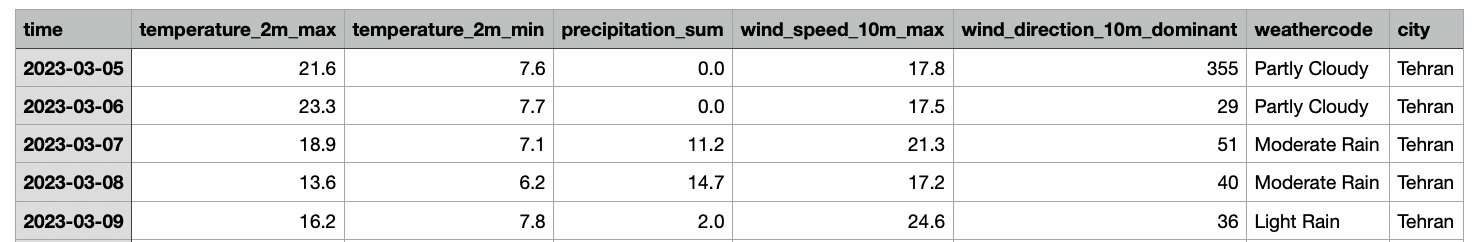
\includegraphics[width=.9\textwidth]{weather.png}
    }
    \subfigure[اقامتگاه‌های شهر رامسر در جاباما]{
        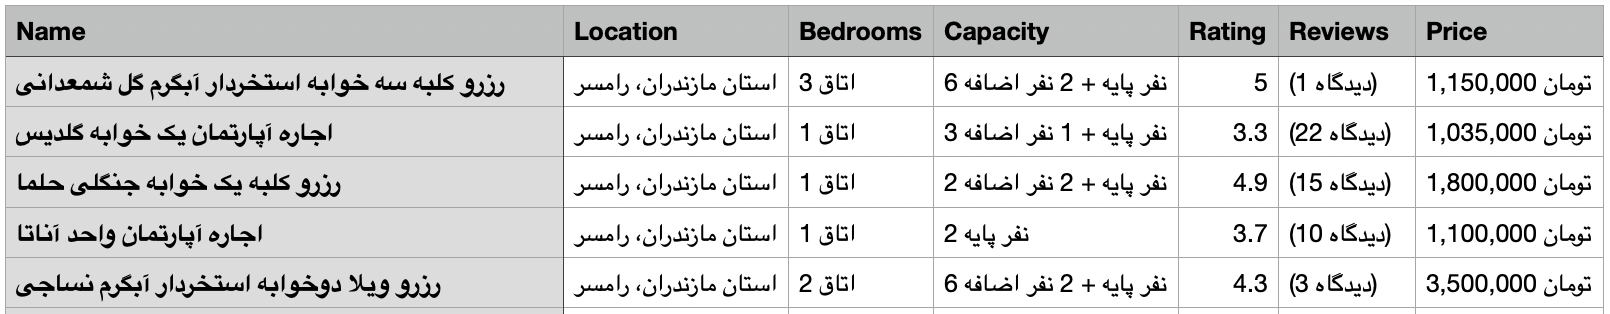
\includegraphics[width=.9\textwidth]{jabama.png}
    }
    \caption{نمونه‌ای از داده‌های استخراج شده}
\end{figure}



\section{روش کار}
مراحل انجام این پژوهش به شرح زیر است:
\begin{enumerate}
    \item \textbf{پیش‌پردازش داده‌ها:}
        \begin{itemize}
            \item بررسی کیفیت و مرتب‌سازی داده‌ها و اصلاح آنها
        \end{itemize}

    \item \textbf{تحلیل اولیه:} 
        \begin{itemize}
            \item تقسیم کشور به ۶-۷ منطقه و بررسی توزیع تردد در هر منطقه
            \item شناسایی پیک سفرهای نوروزی و مقایسه حجم تردد بین مناطق مختلف
        \end{itemize}

    \item \textbf{تحلیل جزئی‌تر:}
        \begin{itemize}
            \item شناسایی محورهای پرتردد و مقایسه بار ترافیکی با ظرفیت جاده‌ها
            \item رتبه‌بندی شهرها بر اساس میزان جذب و ارسال گردشگر
        \end{itemize}
    
        \begin{figure}[htbp]
            \centering
            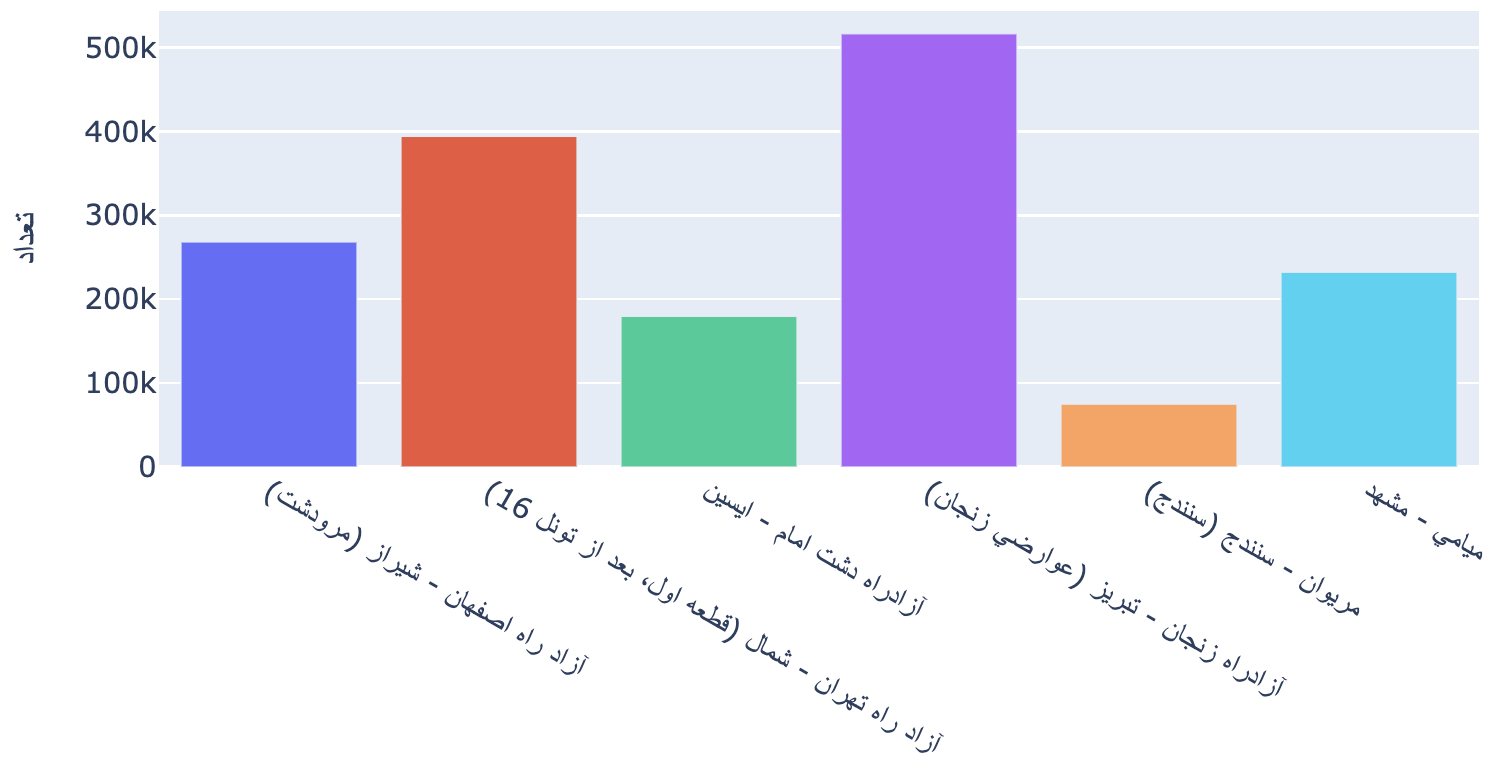
\includegraphics[width=.8\textwidth]{bar-chart.png}
            \caption{مقایسه مجموع تردد سواری برخی محورها در بازه نوروز 1403}
        \end{figure}

        \begin{figure}[htbp]
            \centering
            \subfigure[محور تهران - شمال]{
                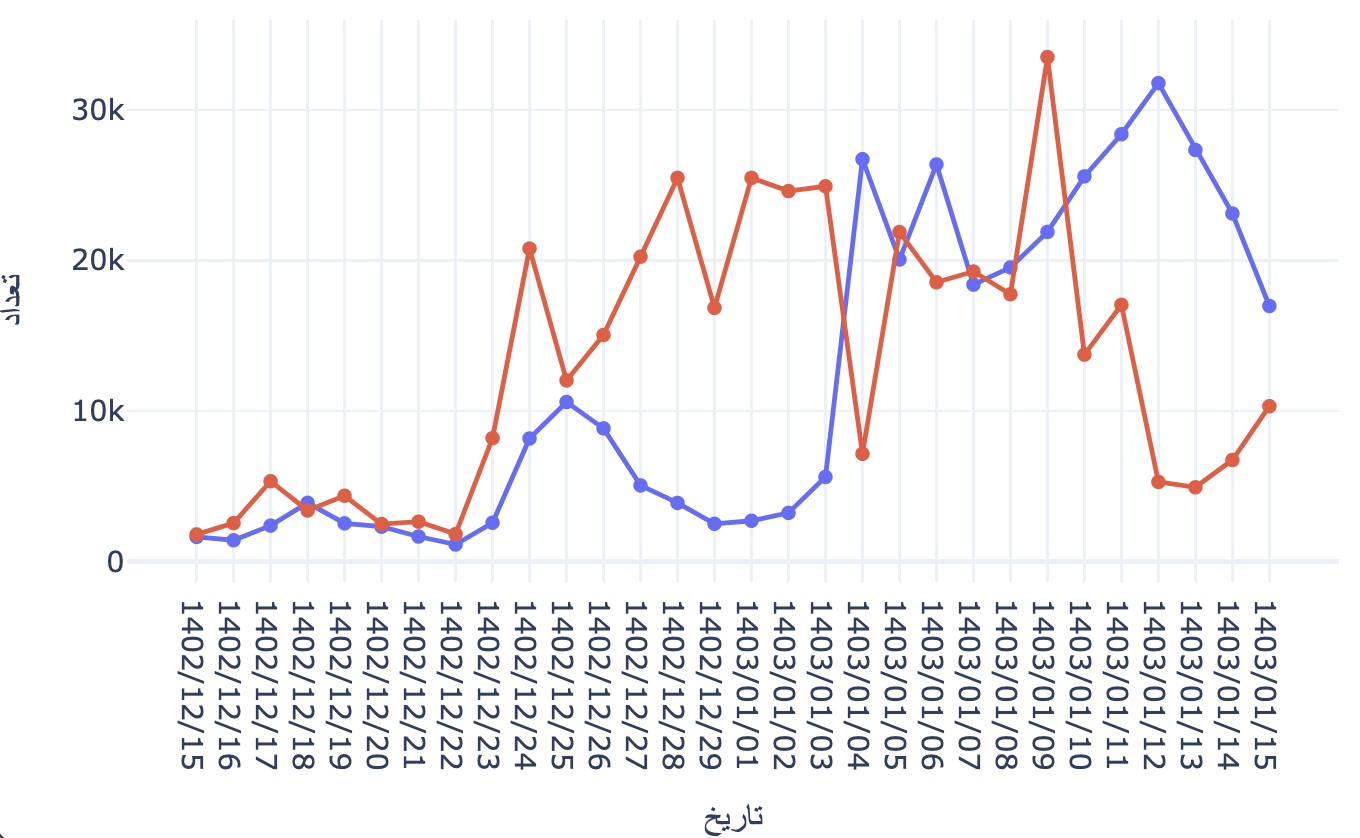
\includegraphics[width=.4\textwidth]{tehran-shomal.png}
            }
            \subfigure[محور اصفهان - شیراز]{
                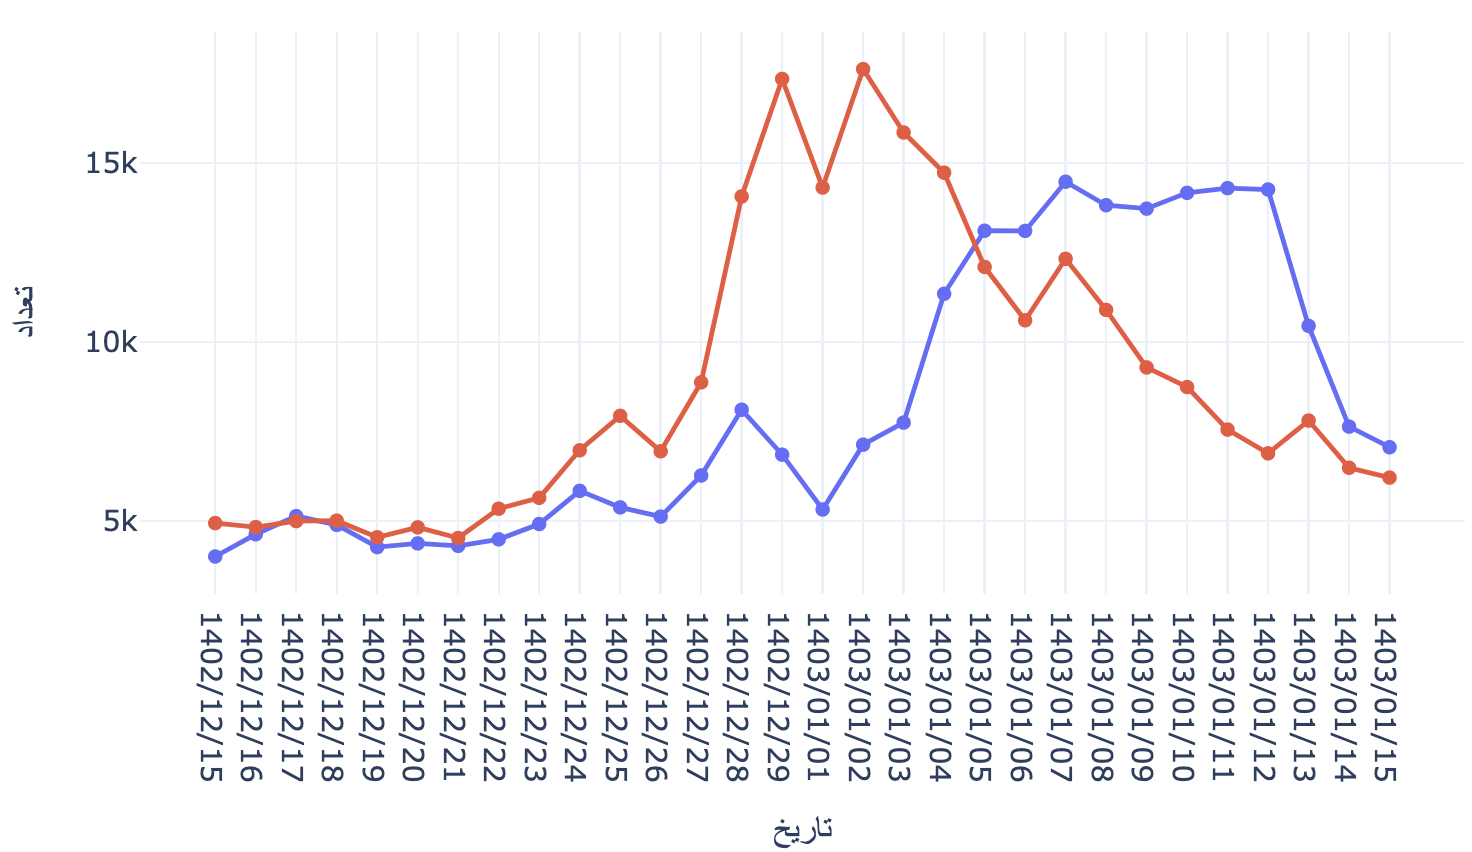
\includegraphics[width=.4\textwidth]{esfahan-shiraz.png}
            }
            \subfigure[محور دشت امام - ایسین]{
                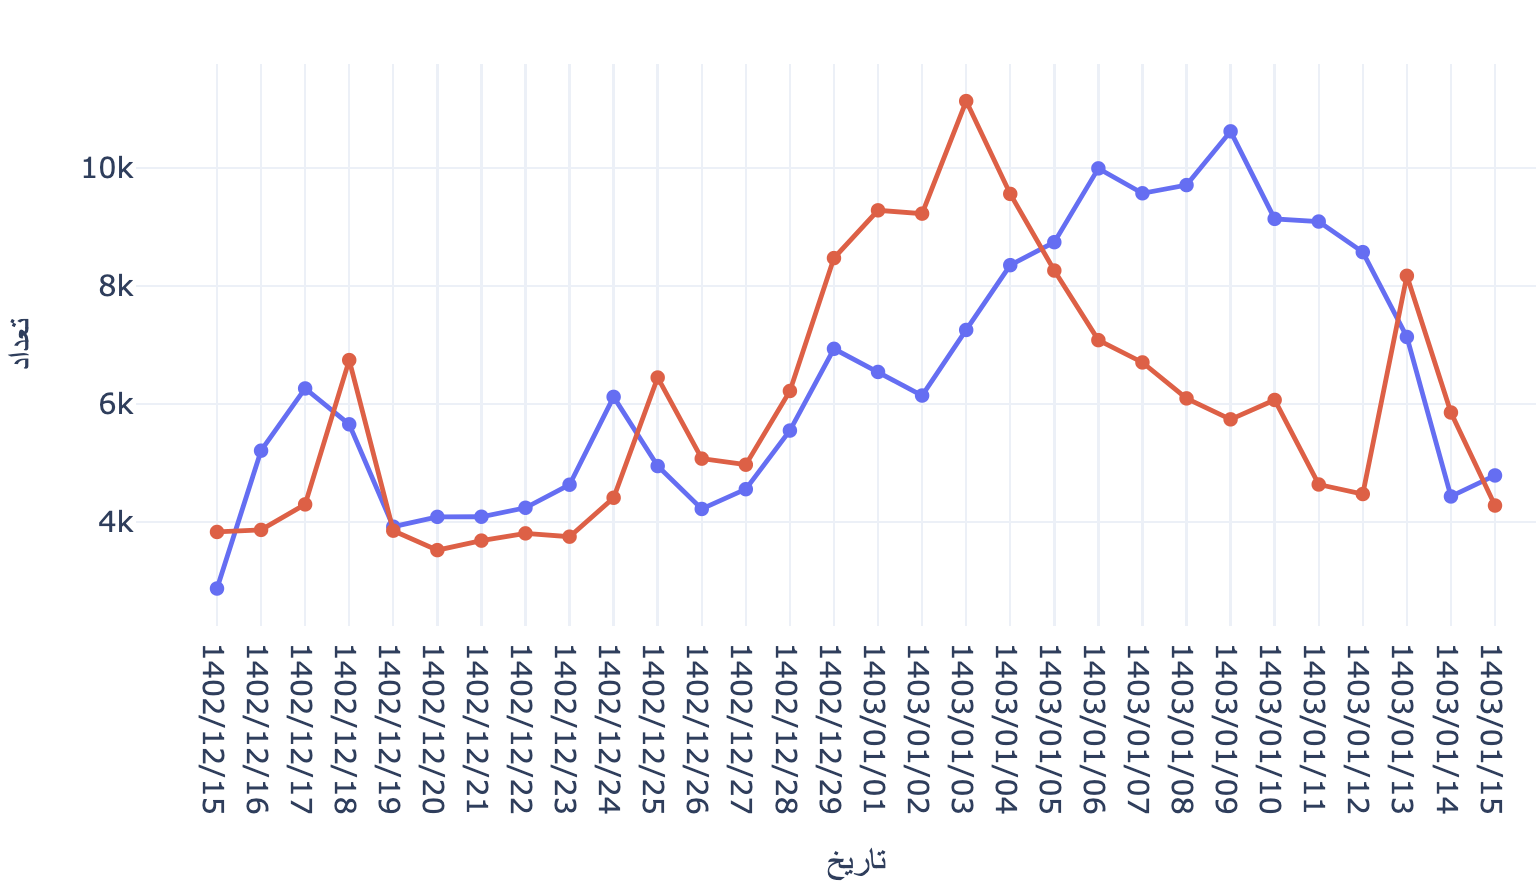
\includegraphics[width=.4\textwidth]{imam-isin.png}
            }
            \subfigure[محور تبریز - زنجان]{
                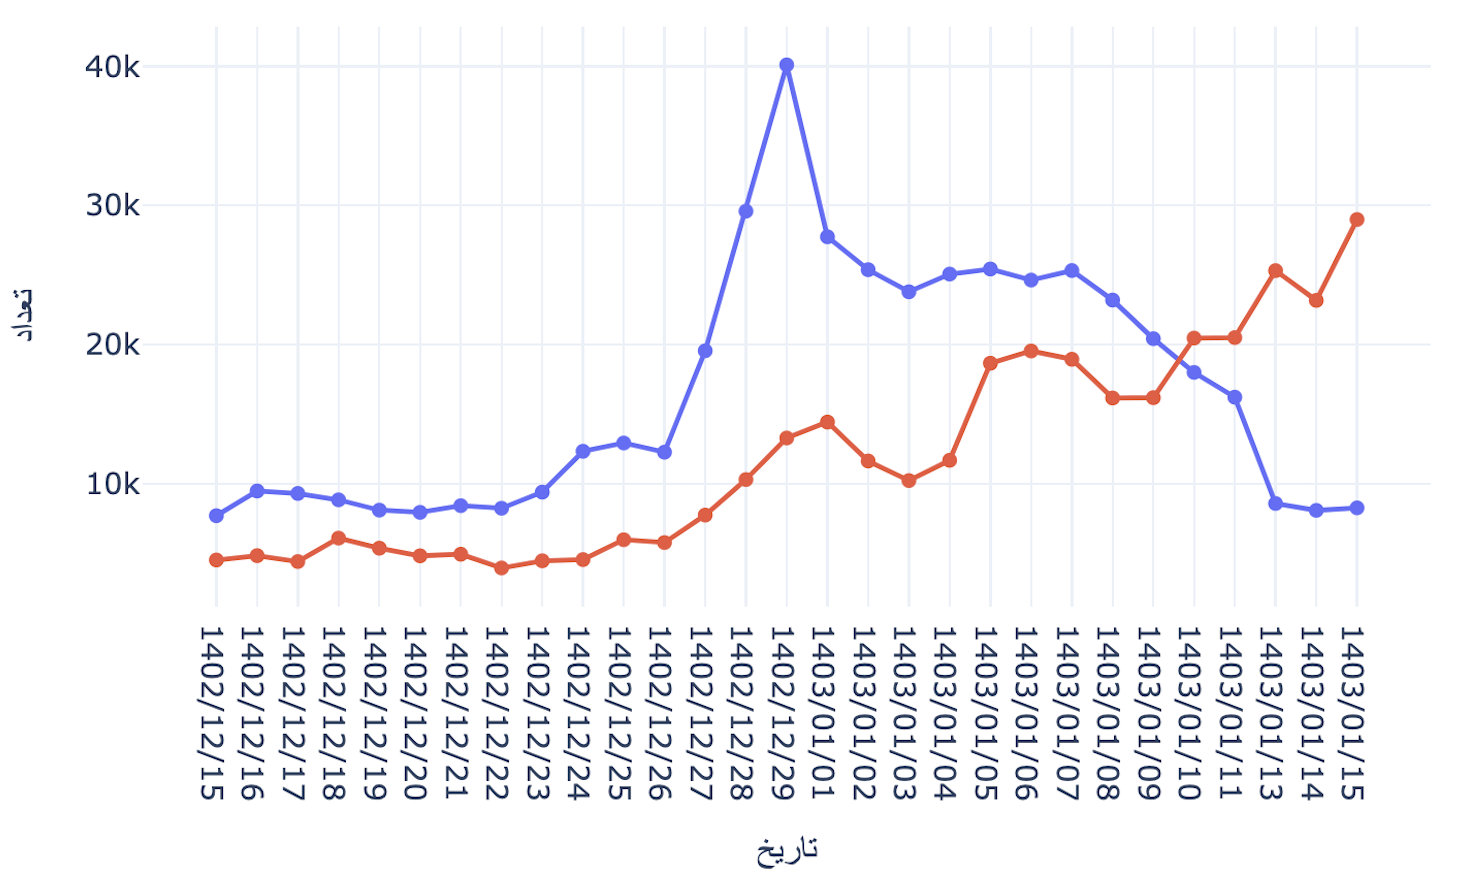
\includegraphics[width=.4\textwidth]{tabriz-zanjan.png}
            }
            \caption{تردد سواری در بازه نوروز 1403 در مسیر رفت (قرمز) و برگشت (آبی) برخی محورها}
        \end{figure}


    \item \textbf{مدل‌سازی و ارائه پیشنهادات:}
        \begin{itemize}
            \item طراحی مدلی برای شناسایی شهرهای با پتانسیل گردشگری بالا
            \item ارائه راهکارهایی برای برنامه‌ریزی و توسعه گردشگری
        \end{itemize}
\end{enumerate}

تمام اعضای تیم در تمامی مراحل همکاری خواهند داشت.


\section{جمع‌بندی}
این پروژه با تحلیل داده‌های تردد جاده‌ای در ایام نوروز و ترکیب آن با اطلاعات تکمیلی، به بررسی الگوهای سفر، مقاصد گردشگری محبوب و مناطق مستعد توسعه گردشگری می‌پردازد. نتایج این پژوهش به سیاست‌گذاران و سرمایه‌گذاران برای بهینه‌سازی مدیریت ترافیک و توسعه صنعت گردشگری کمک می‌کند و گامی مؤثر در جهت آینده‌ای بهتر در این حوزه خواهد بود.

\section{اعضای گروه}
\begin{itemize}
    \item پریساسادات موسوی - 401100239
    \item مهدی طاهری جانبازلو - 401100422
    \item محمد برکتین - 401100082
\end{itemize}

\end{document}